\section{Conversion of Regression Model Outputs to Classification Model Outputs for Anchors Explanation}
\label{app:anchors}


\begin{algorithm}[htbp]
   \caption{Softmax-over-Distance Probability Mapping}
   \label{alg:softmax_distance}
   \begin{algorithmic}[1]
     \Require $r$ \Comment{scalar or vector with values in $[0,6]$}
     \Require $T>0$         \Comment{temperature parameter}
     \Ensure $p$            \Comment{probabilities over $\{0,\dots,6\}$}
     \State $\mathbf{r} \gets \texttt{as\_array}(r)$
     \If{$\exists\,x\in \mathbf{r}\colon x<0\,$ or $\,x>6$}
       \State \textbf{error} “All $r$ values must lie in $[0,6]$.”
     \EndIf
     \State reshape $\mathbf{r}$ into a flat vector $\mathbf{r}_{\mathrm{flat}}$
     \Comment{now of length $n$}
     \State $\mathbf{I} \gets [0,1,2,3,4,5,6]$
     \State \Comment{Compute pairwise distances:}
     \For{$i=1$ to $n$}
       \For{$j=0$ to $6$}
         \State $D_{i,j} \gets \bigl|\mathbf{r}_{\mathrm{flat}}[i] - j\bigr|$
       \EndFor
     \EndFor
     \State \Comment{Form logits by negating and scaling distances:}
     \State $L_{i,j} \gets -\,D_{i,j}\,/\,T \quad\forall\,i,j$
     \State \Comment{Apply numerically-stable softmax row-wise:}
     \For{$i=1$ to $n$}
       \State $m \gets \max_{j}(L_{i,j})$
       \For{$j=0$ to $6$}
         \State $e_{i,j} \gets \exp\bigl(L_{i,j} - m\bigr)$
       \EndFor
       \State $S \gets \sum_{j=0}^{6} e_{i,j}$
       \For{$j=0$ to $6$}
         \State $p_{i,j} \gets e_{i,j} / S$
       \EndFor
     \EndFor
     \State \Comment{Reshape output:}
     \If{$r$ was scalar}
       \State \Return $p_{1,\ast}$    \Comment{single length-7 vector}
     \Else
       \State reshape $p$ to shape $(\text{shape}(r),7)$
       \State \Return $p$
     \EndIf
   \end{algorithmic}
\end{algorithm}


The Algorithm \ref{alg:softmax_distance} serves to convert any real input \(r\in[0,6]\) into a probability distribution over the integer grid \(\{0,1,\dots,6\}\). This approach leverages the intuitive concept of “distance to integer” as a foundation for probabilistic assignment, while carefully controlling numerical precision via temperature scaling and softmax stabilization. This yields a flexible mechanism to interpolate between hard rounding (very small \(T\)) and uniform uncertainty (large \(T\)), all within a rigorously safe and shape-preserving framework. The inspiration for this algorithm comes from \cite{murphy_machine_2012}.




\section{MLP model hyperparameters}
\label{sec:mlp_hyperparameters}

\begin{table}[htbp]
   \centering
   \caption{Search values (or limits) for parameters during hyperparameter optimisation of the Depression Dataset for the monolithic models. (N.A. means Not Applicable)}
   \label{tab:optimiser_values}
   \begin{tabular}{|c|ccc|}
     \hline
     \multicolumn{4}{|c|}{\textbf{Monolithic}} \\
     \hline
     \textbf{Hyperparameter} & \textbf{Lower Limit} & \textbf{Upper Limit} & \textbf{Values} \\
     \hline
     Number of layers & 2 & 4 & N.A \\
     Neurons in input layer & 50 & 90 & N.A \\
     Activation & N.A & N.A & tanh, relu, elu, linear \\
     Batch size & N.A & N.A & 4, 6, 8 \\
     \hline
   \end{tabular}
\end{table}

\begin{table}[htbp] 
    \caption{Combinations Yielding the Overall Best Models. \emph{Metric} refers to the metric used to optimise the model hyperparameters, and \emph{Optimiser} refers to the best optimiser (used for hyperparameter optimisation) corresponding to the overall best model. (BA: Balanced Accuracy, F1: F1 score, MAE: Mean Absolute Error, MAPE: Mean Absolute Percentage Error)}
    \newcolumntype{C}{>{\centering\arraybackslash}X}
    \begin{tabularx}{\textwidth}{CCCCC}
    \toprule
    \textbf{Participant} & \textbf{Data Preprocessing} & \textbf{Problem Type} & \textbf{Optimiser} & \textbf{Metric} \\
    \midrule
    1 & Deletion & Classification & DE & BA \\
    10 & Manual Imputation & Classification & Bayesian & F1 \\
    12 & Deletion & Regression & CMA-DE & MAE \\
    14 & Deletion & Regression & PSO & MAE \\
    15 & Manual Imputation & Regression & PSO & MAE \\
    18 & Manual Imputation & Classification & Bayesian & BA \\
    19 & Deletion & Classification & Bayesian & BA \\
    20 & Deletion & Classification & DE & BA \\
    21 & Manual Imputation & Regression & ES & MAE \\
    23 & Manual Imputation & Classification & DE & BA \\
    24 & Automatic Imputation & Classification & Bayesian & F1 \\
    26 & Manual Imputation & Regression & PSO & MAE \\
    28 & Deletion & Classification & PSO & F1 \\
    29 & Deletion & Classification & Bayesian & F1 \\
    \bottomrule
    \end{tabularx}
    \label{tab:best_model_combination}
   \end{table}
   

Table \ref{tab:best_model_combination} shows the combination of data preprocessing methodology, the problem type and the metric used to optimise the model hyperparameters. The optimiser for which we obtain the overall best model is also provided. Table \ref{tab:best_model_parameters} shows the model parameters for the overall best models. It presents the number of neurons in the DNN, the activation used in the layers and the batch size used during the training of the models. The table shows that most models have at least 3 layers (2 hidden layers and one output layer) and use either a ReLU or a Linear activation. However, for participants 15, 18, and 28, the DNN only has one hidden layer. Furthermore, a batch size of six or four samples works best with most participants. 


\begin{table}[htbp] 
 \caption{Parameters of the overall Best Models. \emph{Neurons} column contains the neurons for each layer (hidden + output layers) in the DNN. (ReLU: Rectified Linear Unit, ELU: Exponential Linear Unit, Tanh: Hyperbolic tangent, Linear: No nonlinear activation)}
 \newcolumntype{C}{>{\centering\arraybackslash}X}
 \begin{tabularx}{\textwidth}{CCCCC}
 \toprule
 \textbf{Participant} & \textbf{Neurons} & \textbf{Activation} & \textbf{Batch Size} \\
 \midrule
 1 & \{38, 7\} & ReLU & 6 \\
 10 & \{60, 33, 7\} & Linear & 8 \\
 12 & \{46, 31, 16, 1\} & Linear & 4 \\
 14 & \{30, 20, 10, 1\} & ReLU & 4 \\
 15 & \{48, 1\} & ReLU & 6 \\
 18 & \{52, 7\} & Linear & 6 \\
 19 & \{35, 21, 7\} & Linear & 6 \\
 20 & \{45, 32, 19, 7\} & ELU & 6 \\
 21 & \{50, 25, 1\} & Tanh & 4 \\
 23 & \{36, 21, 7\} & ReLU & 8 \\
 24 & \{51, 29, 7\} & Linear & 6 \\
 26 & \{46, 31, 16, 1\} & ReLU & 4 \\
 28 & \{60, 7\} & ReLU & 8 \\
 29 & \{51, 36, 21, 7\} & ReLU & 4 \\
 \bottomrule
 \end{tabularx}
 \label{tab:best_model_parameters}
\end{table}




\section{Base model hyperparameters}
\label{sec:base_hyperparameters}

The grid search is implemented in Python using a combination of Python libraries. The Scikit-learn \cite{scikit-learn,sklearn_api} library is used for the modelling and further information on the model parameters reported in the following subsections can be found on their API page. 

\begin{enumerate}
    \item \textbf{Adaboost Classifier:} The grid-search parameters are: Estimators: \{50, 100, 200\}, Learning Rate: \{0.5, 1, 2, 10\}, Algorithm: \{'SAMME', 'SAMME.R'\}. The best model parameters for each participant are shown in Table~\ref{tab:best_model_parameters_abc}.
    
    \begin{table}[H] 
       \caption{Parameters of the Adaboost classifier for the best model after grid search.}
       \newcolumntype{C}{>{\centering\arraybackslash}X}
       \begin{tabularx}{\textwidth}{CCCCC}
       \toprule
    \textbf{Participant} & \textbf{Data Preprocessing} & \textbf{Estimators} & \textbf{Learning rate} & \textbf{Algorithm}  \\ 
    \midrule 
    1 & Impute & 200  & 1  & SAMME.R  \\ 
    10 & Preprocessed & 50  & 0.5  & SAMME  \\ 
    12 & Deletion & 100  & 0.5  & SAMME.R  \\ 
    14 & Deletion & 200  & 2  & SAMME.R  \\ 
    15 & Deletion & 200  & 0.5  & SAMME  \\ 
    18 & Impute & 200  & 10  & SAMME  \\ 
    19 & Deletion & 50  & 0.5  & SAMME  \\ 
    20 & Deletion & 200  & 1  & SAMME  \\ 
    21 & Preprocessed & 50  & 2  & SAMME  \\ 
    23 & Impute & 200  & 10  & SAMME.R  \\ 
    24 & Deletion & 50  & 1  & SAMME.R  \\ 
    26 & Impute & 100  & 0.5  & SAMME  \\ 
    28 & Deletion & 50  & 0.5  & SAMME  \\ 
    29 & Deletion & 100  & 1  & SAMME  \\ 
       \bottomrule
       \end{tabularx}
       \label{tab:best_model_parameters_abc}
    \end{table}

    \item \textbf{Adaboost Regressor:} The grid-search parameters are: Estimators: \{50, 100, 200\}, Learning Rate: \{0.5, 1, 2, 10\}, Loss: \{linear, square, exponential\}. The best model parameters for each participant are shown in Table~\ref{tab:best_model_parameters_abr}.
    
    \begin{table}[H] 
       \caption{Parameters of the Adaboost Regressor for the best model after grid search.}
       \newcolumntype{C}{>{\centering\arraybackslash}X}
       \begin{tabularx}{\textwidth}{CCCCC}
       \toprule
       \textbf{Participant} & \textbf{Data Preprocessing} & \textbf{Estimators} & \textbf{Learning rate} & \textbf{Loss}  \\ 
       \midrule 
       1 & Deletion & 50  & 2  & exponential  \\ 
       10 & Preprocessed & 50  & 0.5  & exponential  \\ 
       12 & Deletion & 100  & 1  & square  \\ 
       14 & Deletion & 50  & 0.5  & exponential  \\ 
       15 & Deletion & 200  & 2  & linear  \\ 
       18 & Preprocessed & 50  & 2  & linear  \\ 
       19 & Impute & 50  & 0.5  & linear  \\ 
       20 & Deletion & 200  & 2  & linear  \\ 
       21 & Deletion & 50  & 1  & square  \\ 
       23 & Preprocessed & 200  & 10  & exponential  \\ 
       24 & Deletion & 50  & 1  & square  \\ 
       26 & Preprocessed & 100  & 10  & exponential  \\ 
       28 & Impute & 100  & 10  & exponential  \\ 
       29 & Deletion & 50  & 1  & square  \\ 
       \bottomrule
       \end{tabularx}
       \label{tab:best_model_parameters_abr}
    \end{table}

    \item \textbf{Elasticnet Regressor:} The grid-search parameters are: Alpha: \{0.5, 1, 2, 10\}, L1-Ratio: \{0, 0.5, 1\}, Selection: \{random, cyclic\}. The best model parameters for each participant are shown in Table~\ref{tab:best_model_parameters_enr}.
    
    \begin{table}[H] 
       \caption{Parameters of the Elasticnet Regressor for the best model after grid search.}
       \newcolumntype{C}{>{\centering\arraybackslash}X}
       \begin{tabularx}{\textwidth}{CCCCC}
       \toprule
       \textbf{Participant} & \textbf{Data Preprocessing} & \textbf{Alpha} & \textbf{L1-Ratio} & \textbf{Selection}  \\ 
       \midrule 
       1 & Impute & 2  & 0  & cyclic  \\ 
       10 & Impute & 0.5  & 0  & cyclic  \\ 
       12 & Deletion & 0.5  & 0  & random  \\ 
       14 & Deletion & 0.5  & 0.5  & random  \\ 
       15 & Preprocessed & 10  & 0  & cyclic  \\ 
       18 & Deletion & 1  & 0  & random  \\ 
       19 & Deletion & 1  & 0  & random  \\ 
       20 & Deletion & 2  & 0  & cyclic  \\ 
       21 & Impute & 10  & 0  & cyclic  \\ 
       23 & Deletion & 0.5  & 0.5  & cyclic  \\ 
       24 & Deletion & 10  & 0  & cyclic  \\ 
       26 & Impute & 0.5  & 0  & cyclic  \\ 
       28 & Deletion & 1  & 0  & random  \\ 
       29 & Deletion & 10  & 0  & cyclic  \\ 
       \bottomrule
       \end{tabularx}
       \label{tab:best_model_parameters_enr}
    \end{table}

    \item \textbf{Gradient Boosting Classifier:} The grid-search parameters are: Loss: \{log-loss\}, Learning Rate: \{0.05, 0.1, 1, 10\}, Estimators: \{50, 100, 200\}, Criterion: \{friedman-mse, squared-error\}, CCP-Alpha: \{0.0, 1, 10\}. The best model parameters for each participant are shown in Table~\ref{tab:best_model_parameters_gbc}.
    
    \begin{table}[H] 
       \caption{Parameters of the Gradient Boosting Classifier for the best model after grid search.}
       \newcolumntype{C}{>{\centering\arraybackslash}X}
       \begin{tabularx}{\textwidth}{CCCCCCC}
       \toprule
       \textbf{Participant} & \textbf{Data Preprocessing} & \textbf{Loss} & \textbf{Learning Rate} & \textbf{Estimators} & \textbf{Criterion} & \textbf{CCP-Alpha}  \\ 
       \midrule 
       1 & Deletion & log-loss & 0.05  & 50  & friedman-mse & 0.0  \\ 
       10 & Impute & log-loss & 0.05  & 50  & friedman-mse & 0.0  \\ 
       12 & Deletion & log-loss & 0.05  & 50  & friedman-mse & 0.0  \\ 
       14 & Preprocessed & log-loss & 0.05  & 50  & friedman-mse & 1  \\ 
       15 & Impute & log-loss & 0.05  & 100  & friedman-mse & 10  \\ 
       18 & Deletion & log-loss & 0.05  & 50  & friedman-mse & 0.0  \\ 
       19 & Deletion & log-loss & 0.1  & 200  & friedman-mse & 0.0  \\ 
       20 & Deletion & log-loss & 10  & 100  & squared-error & 0.0  \\ 
       21 & Deletion & log-loss & 0.1  & 50  & squared-error & 1  \\ 
       23 & Preprocessed & log-loss & 0.05  & 200  & squared-error & 1  \\ 
       24 & Deletion & log-loss & 0.1  & 200  & squared-error & 1  \\ 
       26 & Preprocessed & log-loss & 0.05  & 50  & squared-error & 10  \\ 
       28 & Impute & log-loss & 0.05  & 200  & friedman-mse & 1  \\ 
       29 & Preprocessed & log-loss & 0.05  & 50  & squared-error & 1  \\ 
       \bottomrule
       \end{tabularx}
       \label{tab:best_model_parameters_gbc}
    \end{table}

    \item \textbf{Support Vector Regressor:} The grid-search parameters are: C: \{0.1, 1, 5, 10\}, Kernel: \{linear, poly, rbf, sigmoid\}, Degree: \{2, 3, 4, 5\}, Gamma: \{0.1, 1, scale, auto\}. The best model parameters for each participant are shown in Table~\ref{tab:best_model_parameters_svr}.
    
    \begin{table}[H] 
       \caption{Parameters of the Support Vector Regressor for the best model after grid search.}
       \newcolumntype{C}{>{\centering\arraybackslash}X}
       \begin{tabularx}{\textwidth}{CCCCCC}
       \toprule
       \textbf{Participant} & \textbf{Data Preprocessing} & \textbf{C} & \textbf{Kernel} & \textbf{Degree} & \textbf{Gamma}  \\ 
       \midrule 
       1 & Preprocessed & 0.1  & sigmoid  & 0  & auto  \\ 
       10 & Impute & 1  & sigmoid  & 0  & auto  \\ 
       12 & Deletion & 1  & rbf  & 0  & 0.1  \\ 
       14 & Deletion & 5  & rbf  & 0  & auto  \\ 
       15 & Deletion & 0.1  & sigmoid  & 0  & auto  \\ 
       18 & Preprocessed & 5  & sigmoid  & 0  & 0.1  \\ 
       19 & Deletion & 0.1  & sigmoid  & 0  & 0.1  \\ 
       20 & Deletion & 0.1  & poly  & 4  & scale  \\ 
       21 & Preprocessed & 1  & poly  & 4  & scale  \\ 
       23 & Impute & 0.1  & poly  & 2  & auto  \\ 
       24 & Impute & 5  & linear  & 0  & scale  \\ 
       26 & Preprocessed & 0.1  & poly  & 5  & scale  \\ 
       28 & Deletion & 1  & poly  & 2  & scale  \\ 
       29 & Deletion & 1  & poly  & 2  & 0.1  \\ 
          \bottomrule
       \end{tabularx}
       \label{tab:best_model_parameters_svr}
    \end{table}

    \item \textbf{Gradient Boosting Regressor:} The grid-search parameters are: Loss: \{squared-error, absolute-error, huber, quantile\}, Learning Rate: \{0.05, 0.1, 1, 10\}, Estimators: \{50, 100, 200\}, Criterion: \{friedman-mse, squared-error\}, CCP-Alpha: \{0.0, 1, 10\}. The best model parameters for each participant are shown in Table~\ref{tab:best_model_parameters_gbr}.
    
    \begin{table}[H] 
       \caption{Parameters of the Gradient Boosting Regressor for the best model after grid search.}
       \newcolumntype{C}{>{\centering\arraybackslash}X}
       \begin{tabularx}{\textwidth}{CCCCCCC}
       \toprule
       \textbf{Participant} & \textbf{Data Preprocessing} & \textbf{Loss} & \textbf{Learning Rate} & \textbf{Estimators} & \textbf{Criterion} & \textbf{CCP-Alpha}  \\ 
       \midrule 
       1 & Preprocessed & absolute-error & 0.05  & 50  & squared-error & 0.0  \\ 
       10 & Preprocessed & squared-error & 0.05  & 50  & squared-error & 0.0  \\ 
       12 & Deletion & absolute-error & 0.1  & 200  & friedman-mse & 0.0  \\ 
       14 & Impute & huber  & 0.1  & 200  & friedman-mse & 0.0  \\ 
       15 & Preprocessed & absolute-error & 1  & 50  & squared-error & 10  \\ 
       18 & Preprocessed & absolute-error & 1  & 50  & squared-error & 1  \\ 
       19 & Impute & squared-error & 0.05  & 100  & friedman-mse & 0.0  \\ 
       20 & Deletion & absolute-error & 0.05  & 50  & friedman-mse & 1  \\ 
       21 & Deletion & absolute-error & 1  & 100  & squared-error & 10  \\ 
       23 & Impute & absolute-error & 0.1  & 50  & friedman-mse & 10  \\ 
       24 & Deletion & absolute-error & 10  & 50  & friedman-mse & 10  \\ 
       26 & Preprocessed & absolute-error & 1  & 50  & squared-error & 10  \\ 
       28 & Preprocessed & absolute-error & 0.1  & 50  & squared-error & 1  \\ 
       29 & Deletion & absolute-error & 1  & 50  & friedman-mse & 0.0  \\ 
          \hline
       \end{tabularx}
       \label{tab:best_model_parameters_gbr}
    \end{table}

    \item \textbf{Random Forest Classifier:} The grid-search parameters are: Estimators: \{50, 100, 200\}, Criterion: \{gini, entropy, log-loss\}, Max Depth: \{None, 5, 10, 20\}, Min-Samples-split: \{2, 5, 10\}, Max Features: \{sqrt, log2, None\}. The best model parameters for each participant are shown in Table~\ref{tab:best_model_parameters_rfc}.
    
    \begin{table}[H] 
       \caption{Parameters of the Random Forest Classifier for the best model after grid search.}
       \newcolumntype{C}{>{\centering\arraybackslash}X}
       \begin{tabularx}{\textwidth}{CCCCCCC}
       \toprule
       \textbf{Participant} & \textbf{Data Preprocessing} & \textbf{Estimators} & \textbf{Criterion} & \textbf{Max Depth} & \textbf{Min-Samples-Split} & \textbf{Max Features}  \\ 
       \midrule 
       1 & Preprocessed & 200  & log-loss & 10  & 10  & sqrt  \\ 
       10 & Preprocessed & 200  & log-loss & 5  & 2  & None  \\ 
       12 & Deletion & 100  & log-loss & 5  & 2  & None  \\ 
       14 & Deletion & 200  & entropy  & 20  & 2  & sqrt  \\ 
       15 & Deletion & 50  & log-loss & 20  & 5  & log2  \\ 
       18 & Impute & 50  & entropy  & 20  & 5  & None  \\ 
       19 & Deletion & 50  & entropy  & 5  & 2  & None  \\ 
       20 & Deletion & 100  & log-loss & 5  & 5  & sqrt  \\ 
       21 & Deletion & 100  & log-loss & None  & 2  & sqrt  \\ 
       23 & Deletion & 200  & entropy  & 5  & 10  & log2  \\ 
       24 & Deletion & 200  & log-loss & 20  & 5  & None  \\ 
       26 & Deletion & 100  & gini  & 5  & 5  & log2  \\ 
       28 & Deletion & 200  & gini  & 5  & 10  & sqrt  \\ 
       29 & Deletion & 200  & gini  & 20  & 2  & None  \\ 
          \bottomrule
       \end{tabularx}
       \label{tab:best_model_parameters_rfc}
    \end{table}

    \item \textbf{Poisson Regressor:} The grid-search parameters are: Alpha: \{0.5, 1, 2, 10\}, Solver: \{lbfgs, newton-cholesky\}, Max-Iteration: \{100, 200, 500\}. The best model parameters for each participant are shown in Table~\ref{tab:best_model_parameters_pr}.
    
    \begin{table}[H] 
       \caption{Parameters of the Poisson Regressor for the best model after grid search.}
       \newcolumntype{C}{>{\centering\arraybackslash}X}
       \begin{tabularx}{\textwidth}{CCCCC}
       \toprule
       \textbf{Participant} & \textbf{Data Preprocessing} & \textbf{Alpha} & \textbf{Solver} & \textbf{Max-Iteration}  \\ 
       \midrule 
       1 & Impute & 10  & lbfgs  & 500  \\ 
       10 & Impute & 2  & lbfgs  & 200  \\ 
       12 & Deletion & 2  & lbfgs  & 500  \\ 
       14 & Impute & 1  & newton-cholesky  & 200  \\ 
       15 & Deletion & 10  & lbfgs  & 500  \\ 
       18 & Preprocessed & 10  & newton-cholesky  & 100  \\ 
       19 & Deletion & 2  & lbfgs  & 500  \\ 
       20 & Deletion & 10  & lbfgs  & 500  \\ 
       21 & Deletion & 10  & lbfgs  & 200  \\ 
       23 & Preprocessed & 10  & newton-cholesky  & 500  \\ 
       24 & Deletion & 10  & lbfgs  & 500  \\ 
       26 & Impute & 2  & lbfgs  & 500  \\ 
       28 & Impute & 2  & lbfgs  & 200  \\ 
       29 & Deletion & 10  & newton-cholesky  & 200  \\ 
       \bottomrule
       \end{tabularx}
       \label{tab:best_model_parameters_pr}
    \end{table}

    \item \textbf{Support Vector Classifier:} The grid-search parameters are: C: \{0.1, 1, 5, 10\}, Kernel: \{linear, poly, rbf, sigmoid\}, Degree: \{2, 3, 4, 5\}, Gamma: \{0.1, 1, scale, auto\}. The best model parameters for each participant are shown in Table~\ref{tab:best_model_parameters_svc}.
    
    \begin{table}[H] 
       \caption{Parameters of the Support Vector Classifier for the best model after grid search.}
       \newcolumntype{C}{>{\centering\arraybackslash}X}
       \begin{tabularx}{\textwidth}{CCCCCC}
       \toprule
       \textbf{Participant} & \textbf{Data Preprocessing} & \textbf{C} & \textbf{Kernel} & \textbf{Degree} & \textbf{Gamma}  \\ 
       \midrule 
       1 & Preprocessed & 5  & poly  & 2  & auto  \\ 
       10 & Preprocessed & 10  & rbf  & 0  & 0.1  \\ 
       12 & Deletion & 1  & sigmoid  & 0  & 0.1  \\ 
       14 & Deletion & 0.1  & linear  & 0  & scale  \\ 
       15 & Preprocessed & 0.1  & rbf  & 0  & auto  \\ 
       18 & Impute & 0.1  & poly  & 2  & scale  \\ 
       19 & Deletion & 5  & linear  & 0  & auto  \\ 
       20 & Deletion & 1  & sigmoid  & 0  & auto  \\ 
       21 & Preprocessed & 1  & poly  & 4  & auto  \\ 
       23 & Deletion & 0.1  & sigmoid  & 0  & scale  \\ 
       24 & Impute & 10  & rbf  & 0  & scale  \\ 
       26 & Preprocessed & 0.1  & rbf  & 0  & auto  \\ 
       28 & Preprocessed & 1  & rbf  & 0  & scale  \\ 
       29 & Deletion & 5  & poly  & 4  & scale  \\ 
          \bottomrule
       \end{tabularx}
       \label{tab:best_model_parameters_svc}
    \end{table}

    \item \textbf{Random Forest Regressor:} The grid-search parameters are: Estimators: \{50, 100, 200\}, Criterion: \{squared-error, absolute-error, friedman-mse, poisson\}, Max Depth: \{None, 5, 10, 20\}, Min-Samples-split: \{2, 5, 10\}, Max Features: \{sqrt, log2, None\}. The best model parameters for each participant are shown in Table~\ref{tab:best_model_parameters_rfr}.
    
    \begin{table}[H] 
       \caption{Parameters of the Random Forest Regressor for the best model after grid search.}
       \newcolumntype{C}{>{\centering\arraybackslash}X}
       \begin{tabularx}{\textwidth}{CCCCCCC}
       \toprule
       \textbf{Participant} & \textbf{Data Preprocessing} & \textbf{Estimators} & \textbf{Criterion} & \textbf{Max Depth} & \textbf{Min-Samples-Split} & \textbf{Max Features}  \\ 
       \midrule 
       1 & Impute & 50  & absolute-error & 5  & 2  & log2  \\ 
       10 & Impute & 200  & poisson  & 5  & 10  & None  \\ 
       12 & Deletion & 50  & friedman-mse & 10  & 5  & log2  \\ 
       14 & Deletion & 50  & absolute-error & 10  & 5  & log2  \\ 
       15 & Preprocessed & 50  & squared-error & None  & 10  & log2  \\ 
       18 & Deletion & 50  & absolute-error & 5  & 2  & log2  \\ 
       19 & Preprocessed & 50  & poisson  & 20  & 2  & sqrt  \\ 
       20 & Deletion & 50  & poisson  & 10  & 5  & sqrt  \\ 
       21 & Deletion & 50  & absolute-error & 20  & 10  & log2  \\ 
       23 & Deletion & 100  & absolute-error & 5  & 2  & log2  \\ 
       24 & Deletion & 50  & absolute-error & 5  & 10  & log2  \\ 
       26 & Preprocessed & 200  & absolute-error & 5  & 2  & log2  \\ 
       28 & Preprocessed & 200  & absolute-error & 5  & 10  & sqrt  \\ 
       29 & Deletion & 50  & friedman-mse & 5  & 2  & sqrt  \\ 
          \bottomrule
       \end{tabularx}
       \label{tab:best_model_parameters_rfr}
    \end{table}
\end{enumerate}




\section{Compositional Model Information}
\label{sec:compositional_model_information}

\subsection{Model Features}
\label{sec:appendix_model_features}
\textbf{The following are the input features for each cluster model used in Approach 1.}
\begin{enumerate}
    \item Diet: past\_day\_fats, past\_day\_sugars, past\_day\_caffeine, time\_of\_day
    \item Activity: cumm\_step\_calorie, cumm\_step\_distance, cumm\_step\_count, exercise\_calorie, exercise\_duration, time\_of\_day
    \item Physiological: heart\_rate, ppg\_std, MeanBreathingTime, Consistency, time\_of\_day (excluding deleted columns)
    \item Psychological: distracted, anxious, time\_of\_day
    \item Neurocognitive: gw\_consistency, gw\_efficiency, mf\_consistency, mf\_efficiency, ls\_span, ls\_consistency, ls\_efficiency, fo\_consistency\_all, fo\_efficiency\_all, MeanBreathingTime\_TT, Consistency\_TT, LD\_RareG\_diff, LD\_GL\_bias, gw\_leftDLPFC, mf\_leftDLPFC, ls\_leftDLPFC, fo\_leftDLPFC, gw\_dACC, mf\_dACC, ls\_dACC, fo\_dACC, TT\_leftDLPFC, TT\_dACC, diff\_rareLG\_leftDLPFC, diff\_rareLG\_dACC, GLbias\_leftDLPFC, GLbias\_dACC, time\_of\_day
    \item Sleep: prev\_night\_sleep, time\_of\_day (excluding deleted columns)
\end{enumerate}

\textbf{The following are the input features for each cluster model used in Approach 2.}
\begin{enumerate}
    \item Discrete: anxious, distracted, past\_day\_fats, past\_day\_sugars, past\_day\_caffeine, time\_of\_day
    \item Continuous: MeanBreathingTime, Consistency, cumm\_step\_calorie, cumm\_step\_distance, cumm\_step\_count, exercise\_calorie, exercise\_duration, heart\_rate, ppg\_std, prev\_night\_sleep
    \item Neuro: gw\_consistency, gw\_efficiency, mf\_consistency, mf\_efficiency, ls\_span, ls\_consistency, ls\_efficiency, fo\_consistency\_all, fo\_efficiency\_all, MeanBreathingTime\_TT, Consistency\_TT, LD\_RareG\_diff, LD\_GL\_bias, gw\_leftDLPFC, mf\_leftDLPFC, ls\_leftDLPFC, fo\_leftDLPFC, gw\_dACC, mf\_dACC, ls\_dACC, fo\_dACC, TT\_leftDLPFC, TT\_dACC, diff\_rareLG\_leftDLPFC, diff\_rareLG\_dACC, GLbias\_leftDLPFC, GLbias\_dACC
\end{enumerate}

\textbf{The following are the input features for each cluster model used in Approach 3.}

\begin{enumerate}
    \item Diet: past\_day\_fats, past\_day\_sugars, past\_day\_caffeine
    \item EMA (Ecological Momentary Assessment): anxious, distracted, time\_of\_day
    \item Breathing: MeanBreathingTime, Consistency, MeanBreathingTime\_TT, Consistency\_TT
    \item DACC (dorsal Anterior Cingulate Cortex): mf\_dACC, ls\_dACC, fo\_dACC, TT\_dACC, gw\_dACC, GLbias\_dACC, diff\_rareLG\_dACC
    \item DLPFC (Dorsolateral Prefrontal Cortex): mf\_leftDLPFC, ls\_leftDLPFC, fo\_leftDLPFC, TT\_leftDLPFC, gw\_leftDLPFC, GLbias\_leftDLPFC, diff\_rareLG\_leftDLPFC
    \item Efficiency: mf\_efficiency, ls\_efficiency, fo\_efficiency\_all, gw\_efficiency
    \item Consistency: mf\_consistency, ls\_consistency, fo\_consistency\_all, gw\_consistency
    \item LD (Learning/Decision): LD\_RareG\_diff, LD\_GL\_bias
\end{enumerate}


   
\subsection{Model Hyperparameters and Additional Results Tables}
\begin{table}[H] 
 \caption{Search values (or limits) for parameters during hyperparameters optimisation for the compositional models. (N.A. means Not Applicable)}
 \newcolumntype{R}{>{\raggedright\arraybackslash}X}
 \begin{tabularx}{\textwidth}{RRRR}
 \toprule
 \textbf{Hyperparameter} & \textbf{Lower Limit} & \textbf{Upper Limit} & \textbf{Values}\\
 \midrule
 Number of layers & 2 & 4 & N.A\\
 Neurons in input layer & 30 & 60 & N.A \\
 Activation & N.A & N.A & tanh, relu, elu, linear\\
 Batch size & N.A & N.A & 4, 6, 8 \\
 \bottomrule
 \end{tabularx}
 \label{tab:optimiser_values_compositional}
\end{table}



\begin{table}[htbp] 
 \caption{Best merge and cluster models for Approach 1.  Best models at population levels are Neurocognitive, Diet and Physiological, all in stage 1.}
 \newcolumntype{R}{>{\raggedright\arraybackslash}X}
 \begin{tabularx}{\textwidth}{RR}
 \toprule
 \textbf{Participant} & \textbf{Best Merge Model} \\
 \midrule
 ucsd1  & Neurocognititive   \\
ucsd10 & Psychological      \\
ucsd12 & Neurocognititive   \\
ucsd14 & Neurocognititive   \\
ucsd15 & Neurocognititive   \\
ucsd18 & Physiological      \\
ucsd19 & Diet               \\
ucsd20 & Diet               \\
ucsd21 & Physiological      \\
ucsd23 & Diet               \\
ucsd24 & Sleep              \\
ucsd26 & Diet               \\
ucsd28 & Neurocognititive   \\
ucsd29 & Psychological      \\
 \bottomrule
 \end{tabularx}
 \label{tab:approach1_best_all}
\end{table}


\begin{table}[H] 
 \caption{Best merge and cluster models for Approach 2. Best models at population level are Neurocognitive (stage 2) and Continuous (stage 1).}
 \newcolumntype{R}{>{\raggedright\arraybackslash}X}
 \begin{tabularx}{\textwidth}{RRR}
 \toprule
 \textbf{Participant} & \textbf{Best Merge Model} & \textbf{Best Cluster Model} \\
 \midrule
 ucsd1  & Stage1           & Discrete   \\
ucsd10 & Neurocognitive   & Continuous \\
ucsd12 & Neurocognitive   & Continuous \\
ucsd14 & Neurocognitive   & Discrete   \\
ucsd15 & Stage1           & Continuous \\
ucsd18 & Neurocognitive   & Discrete   \\
ucsd19 & Neurocognitive   & Continuous \\
ucsd20 & Neurocognitive   & Continuous \\
ucsd21 & Neurocognitive   & Discrete   \\
ucsd23 & Neurocognitive   & Continuous \\
ucsd24 & Neurocognitive   & Continuous \\
ucsd26 & Neurocognitive   & Discrete   \\
ucsd28 & Neurocognitive   & Continuous \\
ucsd29 & Neurocognitive   & Continuous \\
 \bottomrule
 \end{tabularx}
 \label{tab:approach2_best_all}
\end{table}



\begin{table}[H] 
 \caption{Best merge and cluster models for Approach 3.}
 \newcolumntype{R}{>{\raggedright\arraybackslash}X}
 \begin{tabularx}{\textwidth}{RRR}
 \toprule
 \textbf{Participant} & \textbf{Best Merge Model} & \textbf{Best Cluster Model} \\
 \midrule
 ucsd1  & Neurocognitive       & DAcc      \\
ucsd10 & EMA  & Ema       \\
ucsd12 & EMA & Ema       \\
ucsd14 & Smartwatch  & Sleep     \\
ucsd15 & EMA  & Breathing \\
ucsd18 & EMA  & Ema       \\
ucsd19 & Smartwatch  & Heart     \\
ucsd20 & Smartwatch  & Activity  \\
ucsd21 & Smartwatch  & Heart     \\
ucsd23 & EMA  & Ema       \\
ucsd24 & EMA  & Diet      \\
ucsd26 & EMA  & Diet      \\
ucsd28 & Neurocognitive      & Breathing \\
ucsd29 & SMARTWATCH  & Sleep     \\
 \bottomrule
 \end{tabularx}
 \label{tab:approach3_best_all}
\end{table}





\section{Correlation Plot}
\label{sec:correlation_plot}


\begin{figure}[htbp]
   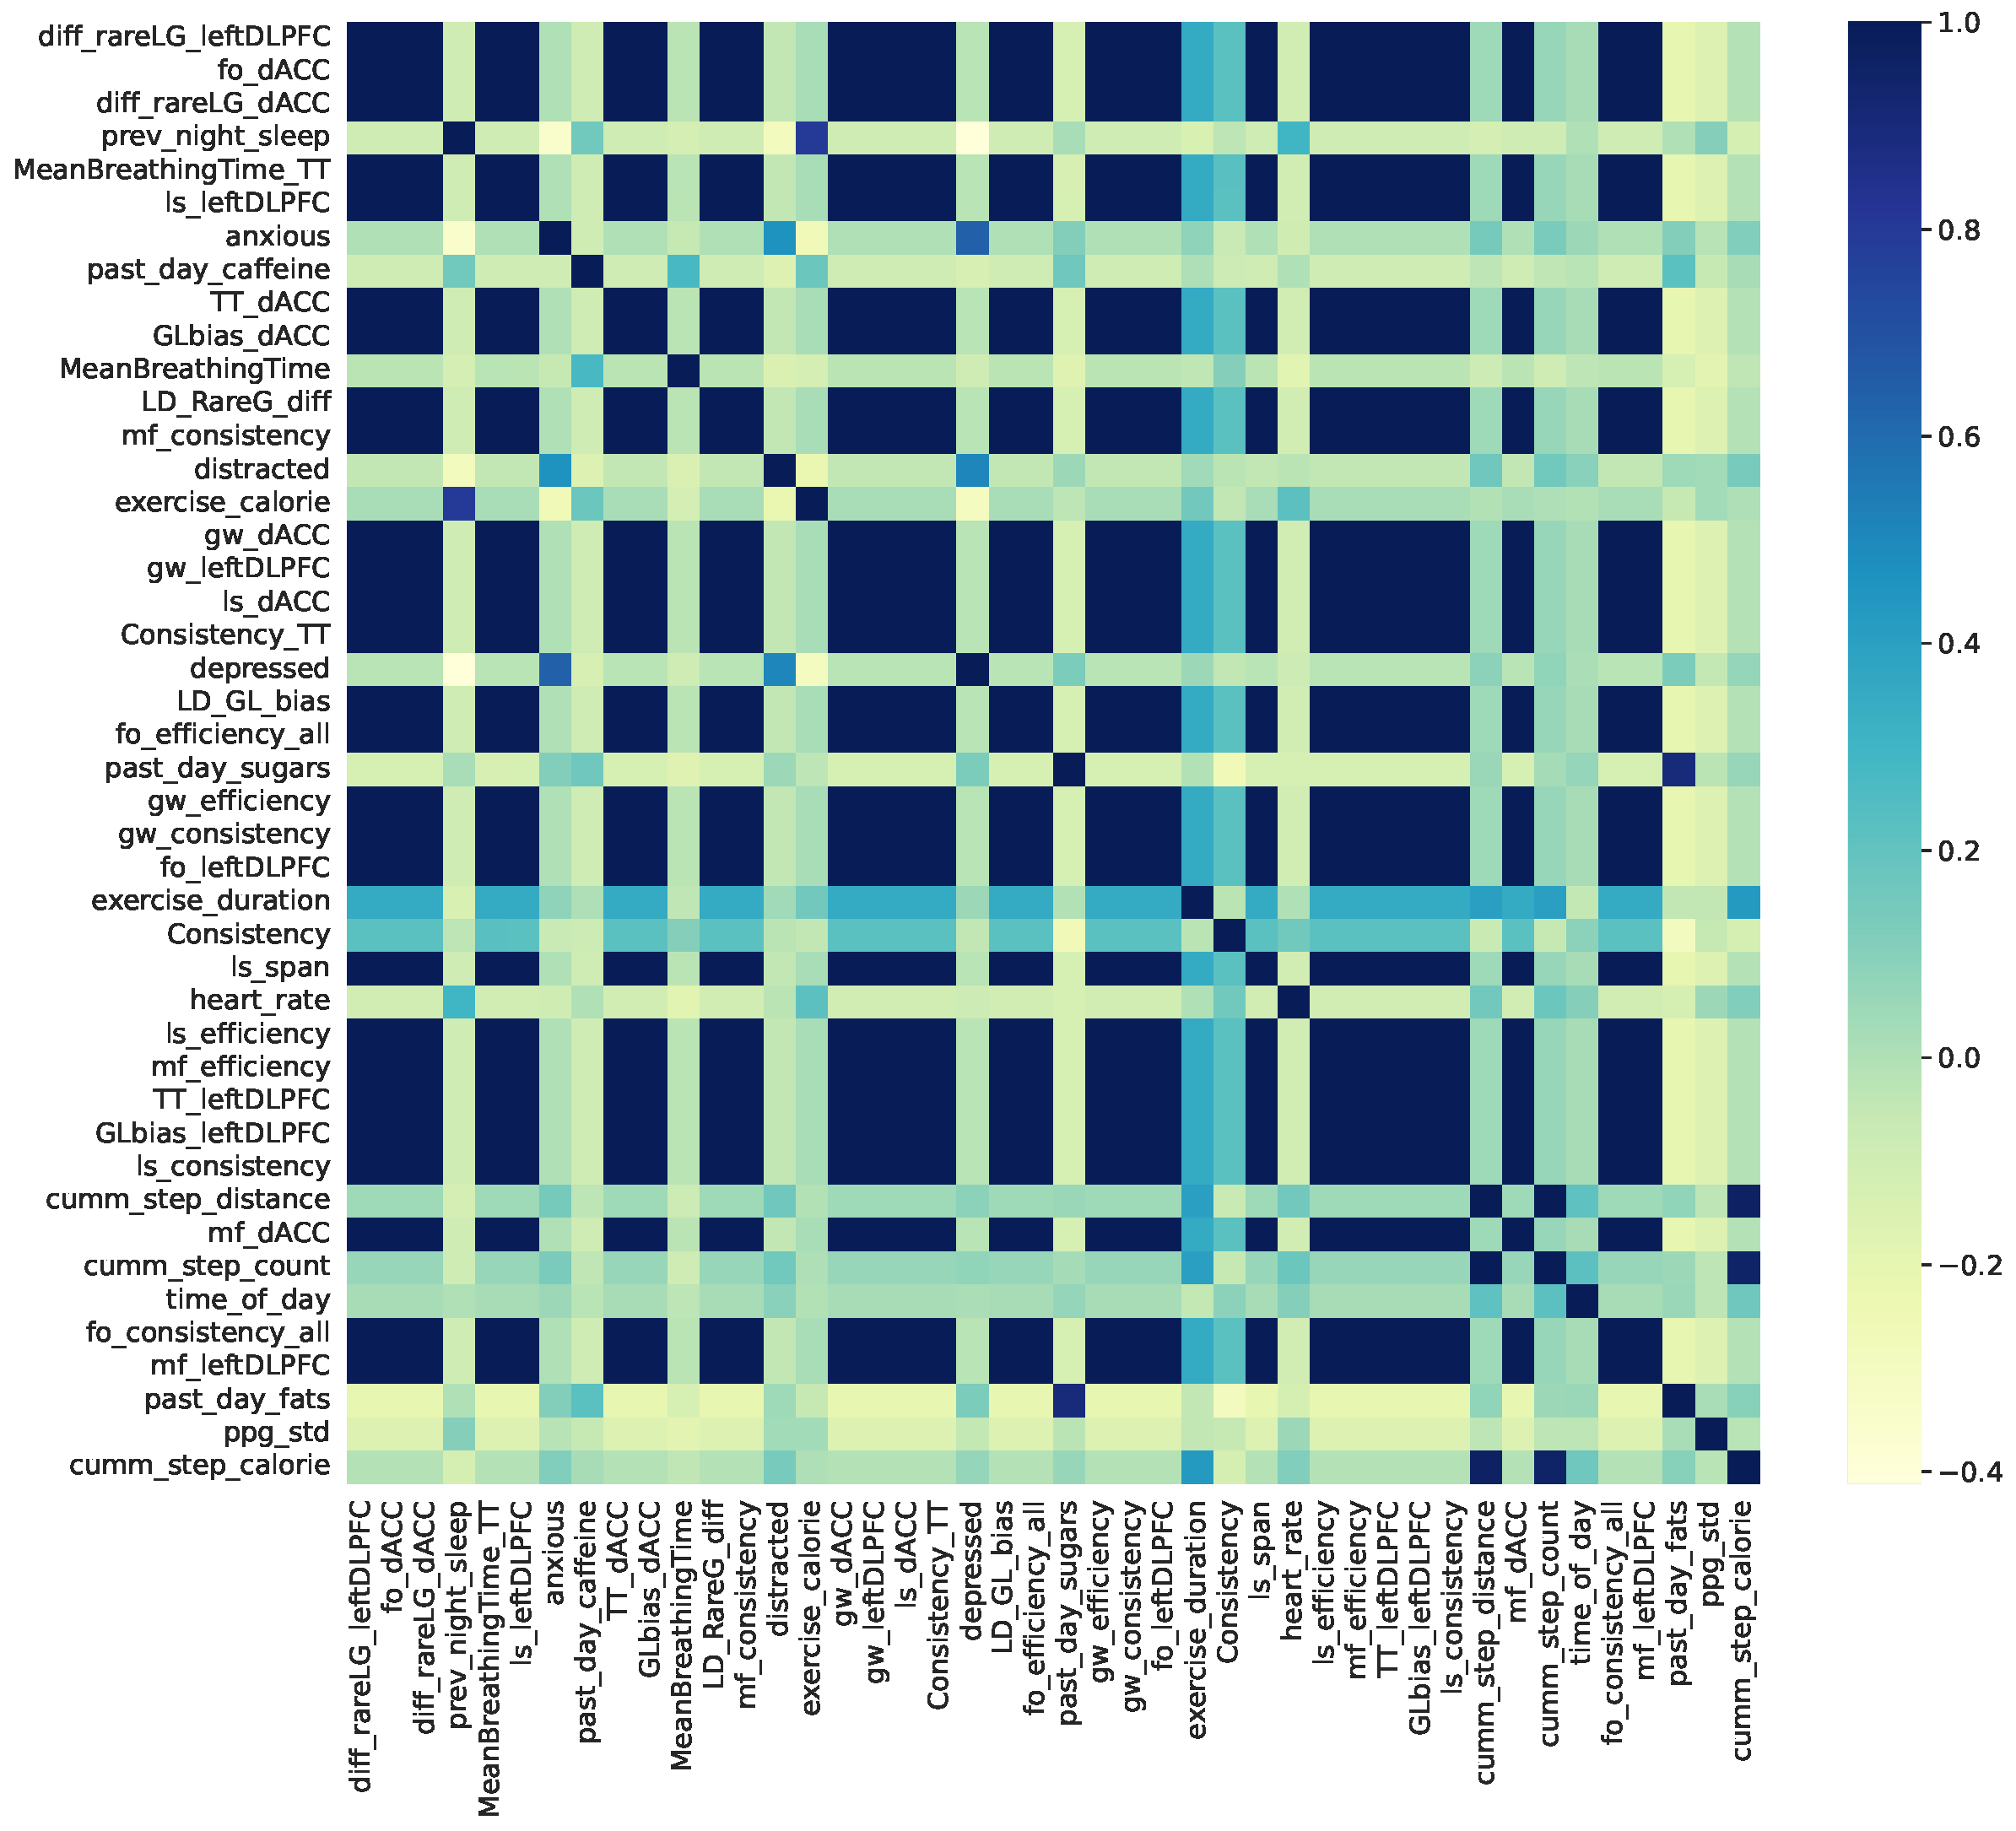
\includegraphics[width = \linewidth]{appendices/fig/spearman_correlation.pdf}
   \caption{The figure shows the correlation plot for all the input features and output feature used in the models with each other. The bar on the right shows which colour corresponds to which value of correlation. We use Spearman Rank correlation.}
   
   \label{fig:corr_plot}
\end{figure}




\section{Additional Plots}
\label{sec:additional_results}


\begin{figure}[H]
      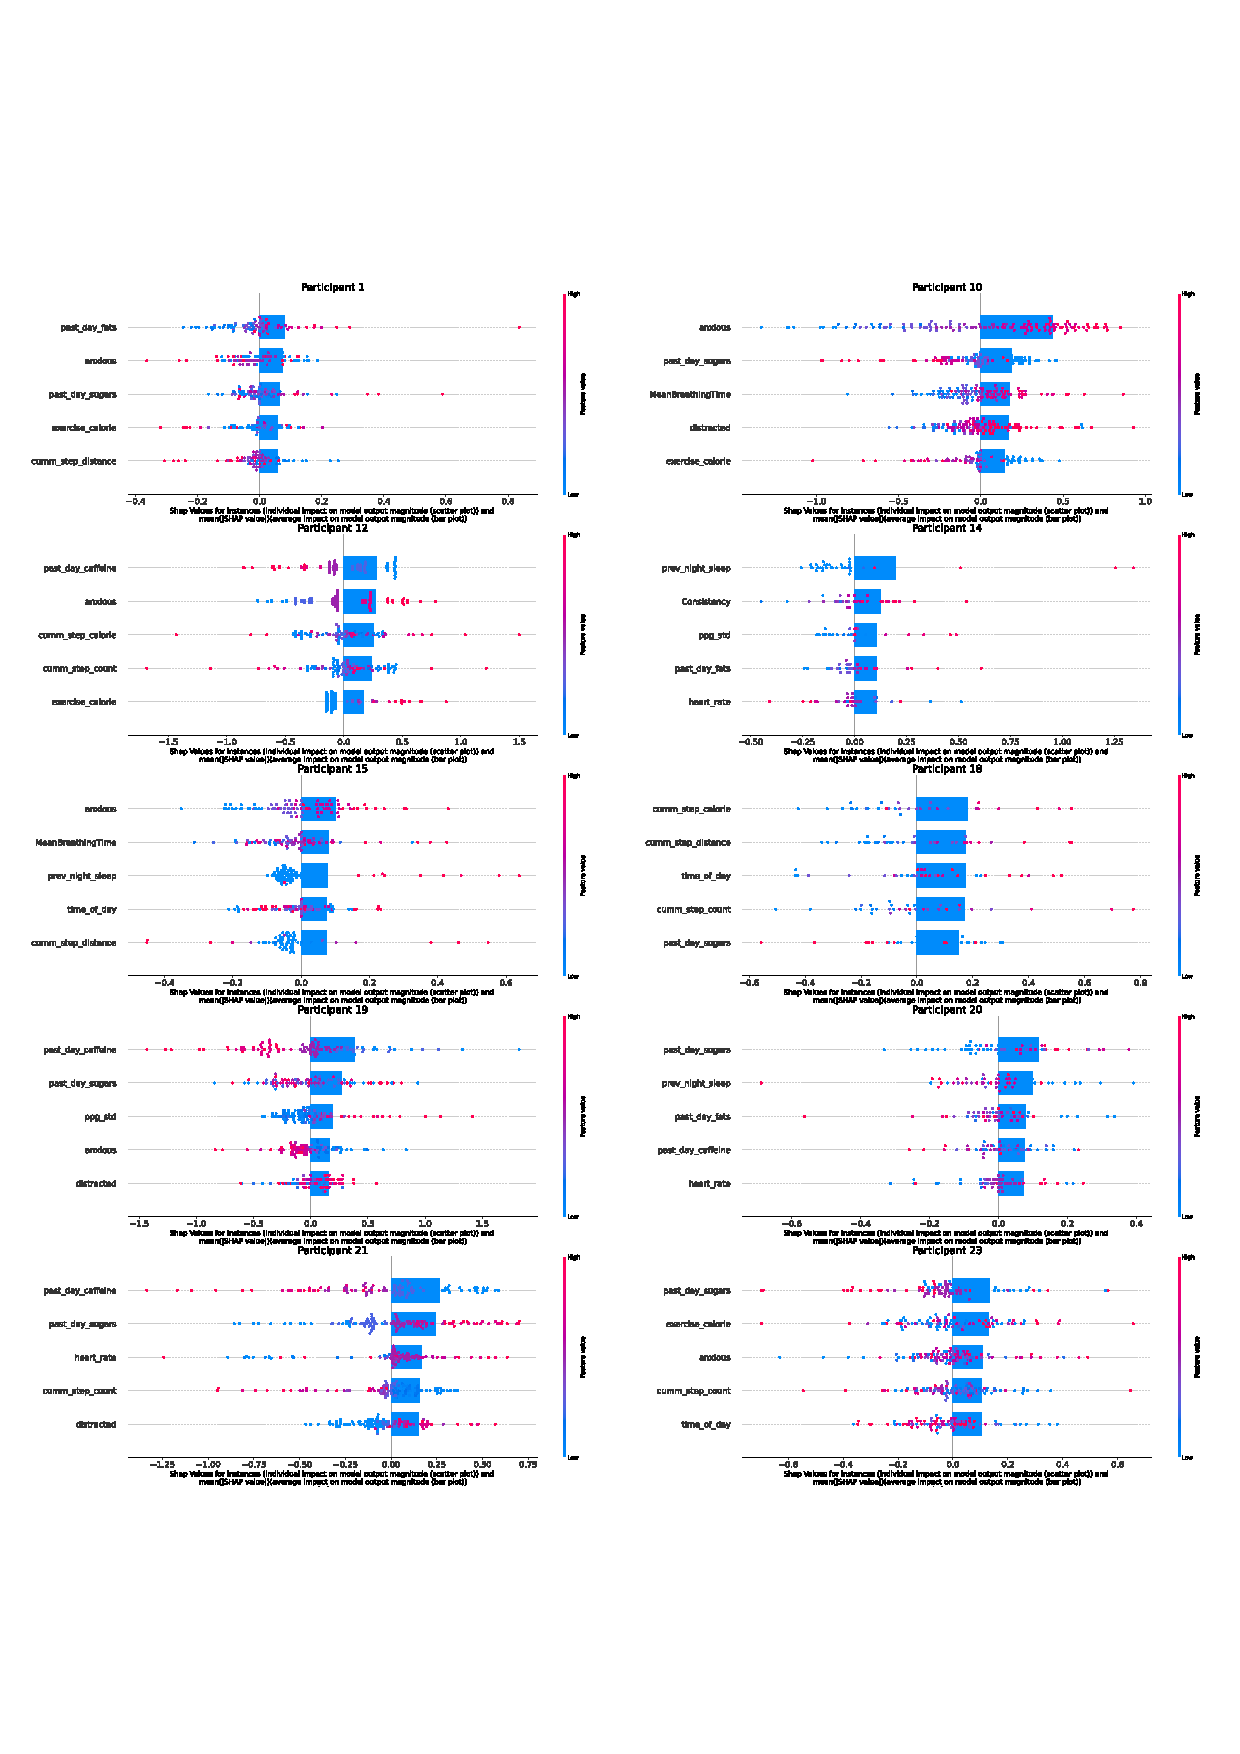
\includegraphics[width = 0.98\linewidth]{appendices/fig/SHAPOverall_1.pdf}

\label{fig:shap_overall_allparts}
\caption{This figure shows the SHAP value effects for the top-5 features in the overall best models for all participants. The scatter plots depict the SHAP values for individual samples, with the colour of the points denoting their magnitude. The bar plots superimposed on top show the mean of the absolute value of the SHAP values over all data points. Figure continues on next page.}
\end{figure}


\begin{figure}[H]
\centering

      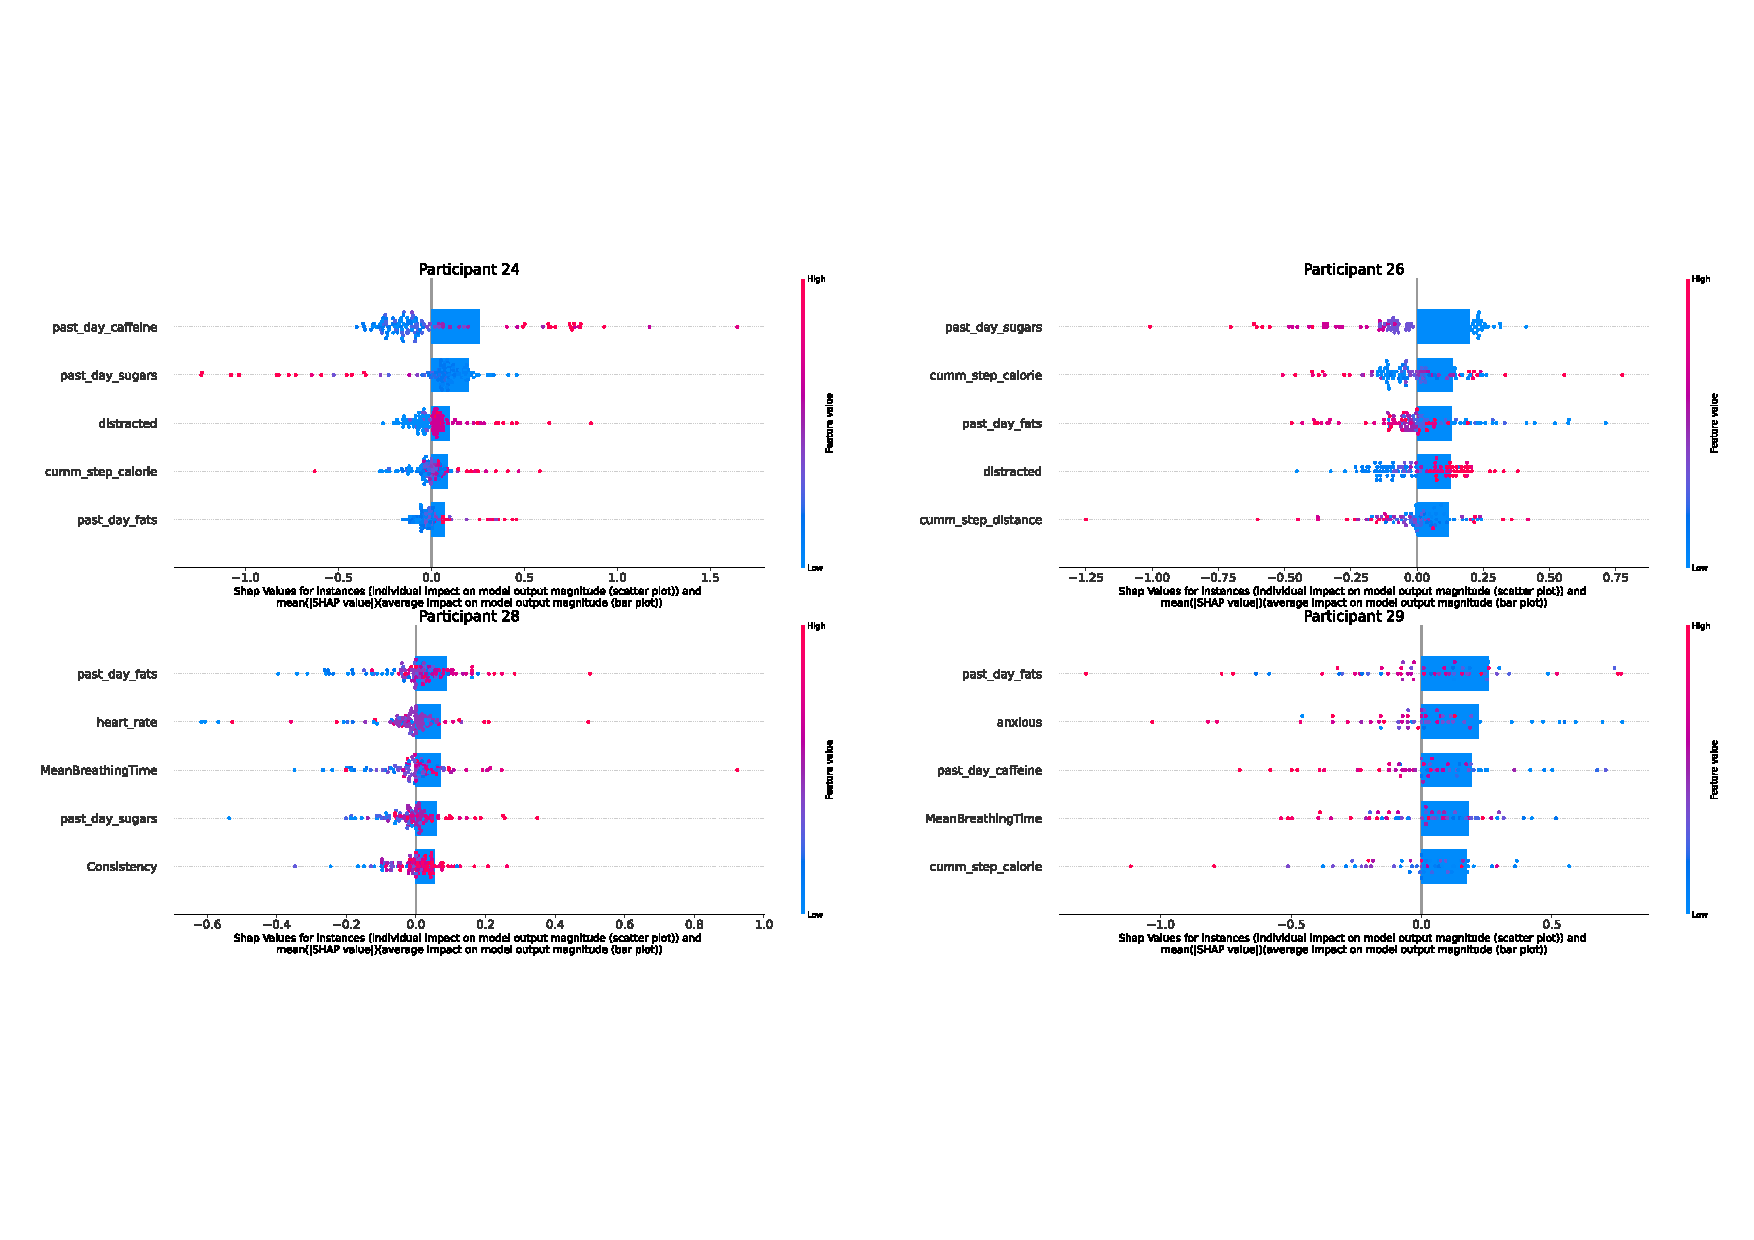
\includegraphics[width = 0.98\linewidth]{appendices/fig/SHAPOverall_2.pdf}
      \caption{Continued from previous page. This figure shows the SHAP value effects for the top-5 features in the overall best models for all participants. The scatter plots depict the SHAP values for individual samples, with the colour of the points denoting their magnitude. The bar plots superimposed on top show the mean of the absolute value of the SHAP values over all data points. Figure continues on next page.}
   \label{fig:shap_overall_allparts}
\end{figure}



\begin{figure}[H]

   \label{fig:ale_overall_all}
   \includegraphics[width = 0.98\linewidth]{appendices/fig/ALEOverall_1.pdf}


\caption{This figure shows the Accumulated Local Effects (ALE) plots for the top-5 features in the overall best models for all participants. The x-axis contains the feature values, and the y-axis contains the ALE values. The ALE values denote the magnitude of the average effect of a feature value on the model output, i.e., the mood score. Figure continues on next page. Figure continues on next page.}
\end{figure}


\begin{figure}[H]
\includegraphics[width = 0.98\linewidth]{appendices/fig/ALEOverall_2.pdf}
   
      \caption{Continued from previous page. This figure shows the Accumulated Local Effects (ALE) plots for the top-5 features in the overall best models for all participants. The x-axis contains the feature values, and the y-axis contains the ALE values. The ALE values denote the magnitude of the average effect of a feature value on the model output, i.e., the mood score. Figure continues on next page.}
\end{figure}